\documentclass[a4paper,11pt]{scrartcl}

\usepackage[ngerman]{babel}
\usepackage[hidelinks]{hyperref}
\usepackage{apacite}
\usepackage{ltablex}
\usepackage{multirow}
\usepackage{gensymb}
\usepackage{amsmath}
\usepackage{amssymb}
\usepackage{graphicx}
\usepackage{pdflscape}
\usepackage{xcolor}
\usepackage{float}
\usepackage{nameref}

\usepackage{fontspec}
    \setmainfont{EB Garamond}
    \setsansfont{Open Sans}
    \setmonofont{Fira Mono}

\setcounter{secnumdepth}{0}
\renewcommand{\baselinestretch}{1.2}

\begin{document}

\author{PREN Gruppe 7}
\title{Konzeptvarianten}
\subtitle{Testat 2}
\date{\today}

\maketitle

\section*{Versionierung}

\def\arraystretch{1.2}
\begin{tabularx}{\linewidth}{|r|l|X|}
\hline
\textsc{Version} & \textsc{Datum} & \textsc{Bemerkung} \\
\hline
0.1 & Do, 03.11.2017 & Zusammentragen der Konzeptvarianten \\
0.2 & Di, 07.11.2017 & Einfügen Nutzwertanalyse, Morphologischer Kasten \\
0.3 & Di, 07.11.2017 & Überarbeitung; Fertigstellung Vorab-Version \\
0.4 & Do, 09.11.2017 & Überarbeitung gemäss Feedback-Gespräch \\
1.0 & Fr, 10.11.2017 & Überarbeitung zur Abgabe \\
1.1 & Do, 14.12.2017 & Kosmetische Anpassungen für Testat 3 \\
1.2 & So, 07.01.2018 & Finale Überarbeitung gemäss Feedback \\
\hline
\end{tabularx}

\newpage

\tableofcontents

\newpage 

\section {Einleitung}

Im ersten Teil des Projekts (bis Semesterwoche 4, Testat 1) wurde die Aufgabenstellung analysiert um daraus Anforderungen abzuleiten. Hierzu wurde eine funktionale Zerlegung vorgenommen, um aus der Gesamtfunktion der umzusetzenden Lösung Teilfunktionen einzelner Komponenten zu ermitteln (siehe \nameref{lbl:FunktionalesBlockschaltbild}, Seite \pageref{lbl:FunktionalesBlockschaltbild}).

Auf Basis dieser funktionalen Zerlegung und der Recherche konnten zu jeder Teilfunktion mehrere Lösungsvarianten gefunden werden, die in einem morphologischen Kasten (siehe \nameref{lbl:MorphologischerKasten}, Seite \pageref{lbl:MorphologischerKasten}) gesammelt wurden.

Mithilfe des morphologischen Kastens wurden unter Definition je eines Leitkriteriums zwei Lösungsvarianten kombiniert. Die beiden Lösungsvarianten werden in diesem Dokument erläutert (siehe \nameref{lbl:Lösungsvarianten}, Seite \pageref{lbl:Lösungsvarianten}) und in einer Nutzwertanalyse (siehe \nameref{lbl:Nutzwertanalyse}, Seite \pageref{lbl:Nutzwertanalyse}) einander gegenübergestellt und bewertet. Auf dieser Basis wird entschieden, welche der beiden Lösungsvarianten für den weiteren Projektverlauf weiterverfolgt und für die spätere Umsetzung konzipiert werden soll.

\newpage

\section{Lösungsvarianten}
\label{lbl:Lösungsvarianten}

Der Morphologischen Kasten (Seite \pageref{lbl:MorphologischerKasten}) dient als Grundlage zur Kombination verschiedener Lösungsvarianten. Statt sämtliche Lösungskombinationen zu evaluieren -- bei vier Komponenten mit je fünf bzw. neun Komponenten mit je vier Lösungsvorschlägen ergäbe das $5^4 \cdot 4^9 = 16'3840'000$ Varianten! -- wurden sogenannte Leitkriterien definiert, etwa \textit{kostengünstigste} oder \textit{technisch anspruchsvollste} Variante. Zu jedem Leitkriterium wurde dann pro Komponente derjenige Lösungsvorschlag ausgewählt, der diesem Kriterium am besten entspricht.
Für die genaueren Evaluation wurden jedoch nur zwei Kombinationen berücksichtigt: Zum einen ist dies die technisch anspruchvollste Variante -- im Folgenden als Variante «High Tech» bezeichnet --, zum anderen ist dies ein Kompromissvorschlag aus verschiedenen Kombinationen -- mangels Leitkriterium im Folgenden als Variante «optimiert» bezeichnet.

\subsection{Variante 1: «High Tech»}

Mit der Variante «High Tech» (Abbildung \ref{fig:hightech}, Seite \pageref{fig:hightech}) wurde eine möglichst ausgeklügelte und technisch anspruchsvolle Lösungsvariante definiert. Vorhandenes Wissen über die einzelnen Komponenten und Erfahrungen damit waren hierbei kein Entscheidungskriterium.

\begin{figure}[H]
    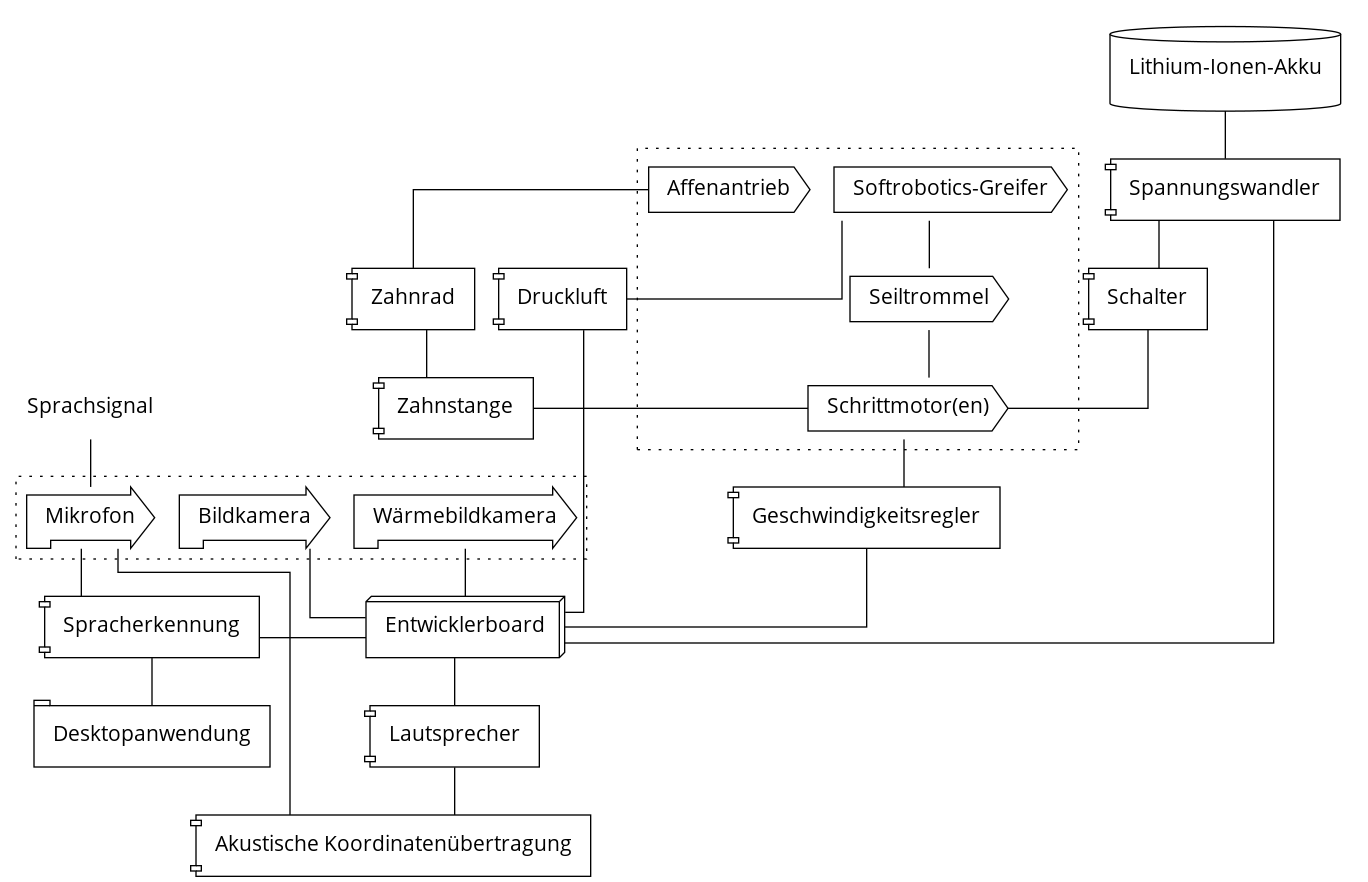
\includegraphics[width=\linewidth]{hightech.png}
    \caption{Hardware-Architektur der Lösungsvariante «High-Tech»}
    \label{fig:hightech}
\end{figure}

\begin{description}
    \item[Softrobotics-Greifer] Diese Idee eintstammt einem YouTube-Video\footnote{\url{https://www.youtube.com/watch?v=uPx8xwRpfFk}}, das eine selbst gefertigte Variante des Greifers und verschiedene Anwendungen dafür zeigt. Der Softrobotics-Greifer ist ein aus Silikon gefertigter, mit Druckluft betriebener Greifmechanismus. Die Innenseite ist mit einem nicht-elastischen, rutschfesten Material beschichtet. Sobald der Greifer aufgeblasen wird, beginnd die Ausdehnung der Aussenseite aus Silikon, und der Greifer schliesst sich. Die rutschfeste Beschichtung sorgt dafür, dass genügend Reibung zwischen dem Greifer und dem Holzwürfel besteht, um diesen zu heben. Für den Betrieb des Greifers ist eine Druckluftzufuhr nötig. Sie muss in der Lage sein, den Überdruck während der Transportzeit des Holzwürfels aufrecht zu erhalten. Beim Abladen der Last muss der Druck ausgeglichen werden können, damit sich der Greifer öffnet. Das Heben und Senken der Last geschieht mit Hilfe eines Elektromotors, der über eine mechanische Schnittstelle mit dem Greifer verbunden ist. Die Signale zum Heben und Senken, sowie Druckaufbau, werden vom Entwicklerboard empfangen. Des weiteren muss dem Board via Sensoren signalisiert werden, wann der Würfel auf-/abgeladen wurde und wie weit der Würfel gehoben wurde.
    \begin{itemize}
        \item Input: Signal zum Greifen/Loslassen, Signal zur vertikalen Bewegung
        \item Output: Greifen/Loslassen abgeschlossen
    \end{itemize}
    \item[Startsignal/Lastkoordinatenübertragung] Das akustische Startsignal wird von einem Mikrofon aufgenommen, per Spracherkennung erkannt und an das Entwicklerboard weitergeleitet. Die Übermittlung der Lastkoordinaten geschieht ebenfalls über ein akustisches Signal. Die durch die Sensoren ermittelte Position wird in ein akustisches Signal umgewandelt, über einen Lautsprecher ausgesendet, mithilfe eines Mikrofons empfangen, per Spracherkennung übersetzt und auf einer Desktopanwendung ausgegeben.
    \begin{itemize}
        \item Input: akustisches Startsignal, elektronische Lastkoordinaten
        \item Output: elektronisches Startsignal, Visualisierung der Lastkoordinaten
    \end{itemize}
    \item[Fortbewegung am Seil] Der Antrieb von \textit{Silisloth} geschieht durch einen «Affenantrieb». Jener besteht aus zwei Schienen, die sich abwechselnd vor- und rückwärts bewegen. Während sich die Schiene eins bewegt, klammert sich Schiene zwei am Drahtseil fest. Ist Schiene eins in Position, klammert sie sich an das Seil und Schiene zwei löst ihren Griff und beginnt sich zu verschieben. Die beiden Schienen werden durch zwei einzelne Elektromotoren entlang der Seilrichtung verschoben. Auch müssen die Schliessmechanismen individuell angesteuert und betrieben werden. Dies geschieht durch einen Elektromotor und unter einer Logik, die das Verschieben und das Lösen und Greifen der Schienen steuert.
    \begin{itemize}
        \item Input: elektronisches Signal Fahren/Halten
    \end{itemize}
    \item[Zielerkennung] Die Wärmebildkamera muss elektronisch dem Entwicklerboard mitteilen können, wo sich die Zielplatte befindet.
    \begin{itemize}
        \item Output: Signal bei Erkennung des Zielfeldes
    \end{itemize}
    \item[Stromversorgung] Der Steuer- und der Laststromkreis werden voneinander getrennt. Somit ist sichergestellt, dass der Steuerkreis garantiert Strom zugeführt bekommt, auch wenn die Motoren betrieben werden. Beide werden durch einen Lithium-Ionen-Akku gespeist.
    \item[Zielmasterkennung] Eine Bildkamera signalisiert \textit{Silisloth}, dass es den Zielmast erreicht hat und die Motoren stoppen müssen.
    \begin{itemize}
        \item Output: Signal bei Erreichen des Mastens
    \end{itemize}
    \item[Lastkoordinatenerfassung] Um die Position der Last an ein Ausgabegerät übertragen zu können, übermittelt eine Bildkamera die Koordinaten an das Entwicklerboard.
    \begin{itemize}
        \item Output: x- und z-Koordinaten als analoges Signal
    \end{itemize}
\end{description}

\subsection{Variante 2: «optimiert»}

Die Variante «optimiert» (Abbildung \ref{fig:optimiert}, Seite \pageref{fig:optimiert}) soll einen Kompromiss zwischen technischem Anspruch und Machbarkeit schliessen. Dabei werden komplizierte Funktionen vereinfacht oder weggelassen. Die Variante soll aber dennoch originell bleiben. Sie sollte weitgehend mit dem vorhandenen Vorwissen umsetzbar sein. Ebenfalls wurde versucht, mögliche Risiken zu minimieren, indem auf erprobte Technologien zurückgegriffen wird.

\begin{figure}[H]
    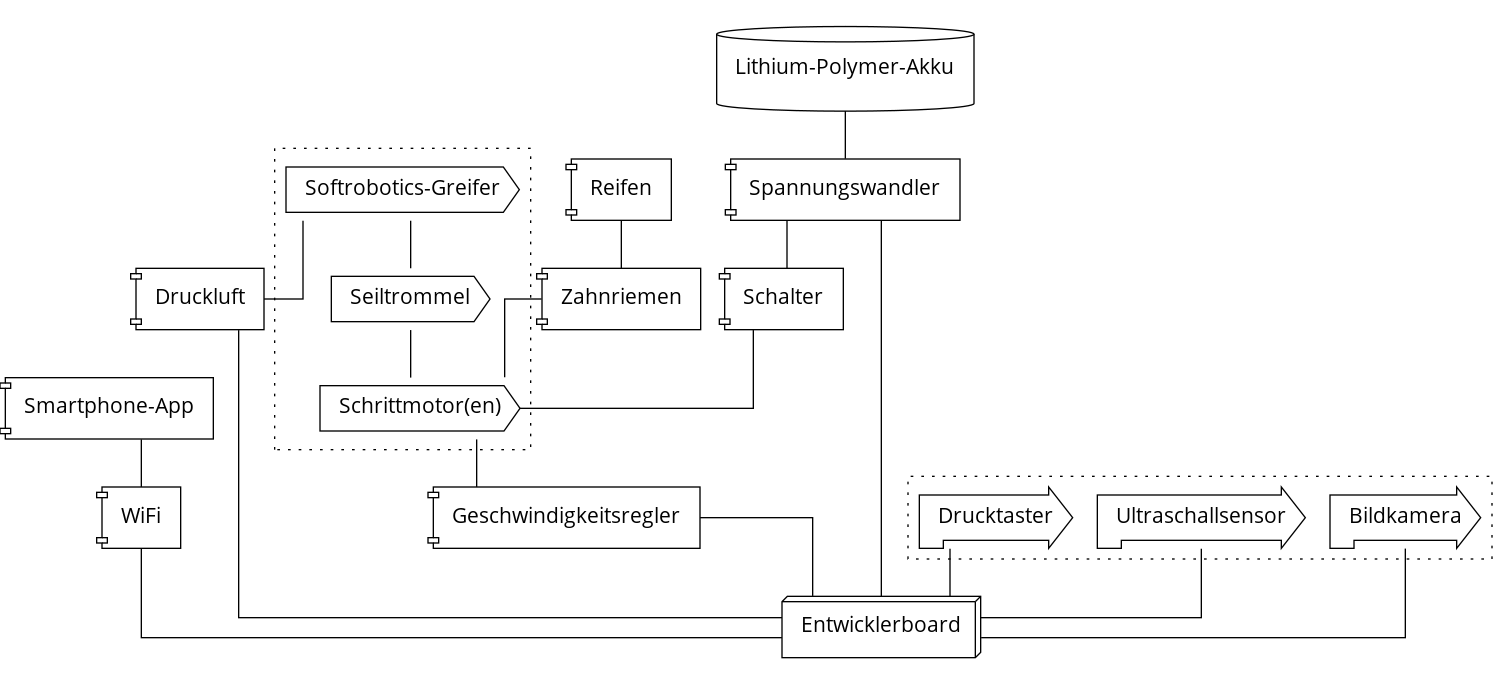
\includegraphics[width=\linewidth]{optimiert.png}
    \caption{Hardware-Architektur der Lösungsvariante «Optimiert»}
    \label{fig:optimiert}
\end{figure}

\begin{description}
    \item [Startsignal/Lastkoordinatenübertragung] Nach dem Count\-down wird auf einer Smart\-phone-App eine Taste betätigt. Das Signal wird via WiFi an \textit{Silisloth} gesendet und dort empfangen und erkannt. Die Koordinaten des Holzwürfels werden von \textit{Silisloth} wieder via WiFi an das Smartphone gesendet und dort visuell dargestellt.
    \begin{itemize}
        \item Input: digitales Startsignal, elektronische Lastkoordinaten
        \item Output: elektronisches Startsignal, Visualisierung der Lastkoordinaten
    \end{itemize}
    \item [Fortbewegung am Seil] Elektromotoren, die von einem Akku gespeist und von einem Entwicklerboard angesteuert werden, treiben Räder an, die via Reibschluss die Kraft übertragen. Die Motoren und der Reibschluss muss in der Lage sein, eine Steigung von 100\% überwinden zu können.
    \begin{itemize}
        \item Input: elektronisches Signal Fahren/Halten
    \end{itemize}
    \item [Zielerkennung] Eine Bildkamera ist zuständig für die Erkennung des Zielfeldes. Nach Erkennung des Feldes wird ein elektronisches Signal an das Entwicklerboard gesendet, welches weiterverarbeitet wird.
    \begin{itemize}
        \item Output: Signal bei Erkennung des Zielfeldes
    \end{itemize}
    \item [Stromversorgung] Der einzige Unterschied zur Variante 1 ist, dass ein Lithium-Polymer-Akku verwendet wird.
    \item [Zielpfostenerkennung] Ein Drucktaster am vordersten Punkt von \textit{Silisloth} sendet bei Berührung mit dem Endpfostens ein Signal an das Entwicklerboard, welches zum Stoppen der Motoren führt.
    \begin{itemize}
        \item Output: Signal bei Berührung es Endpfostens
    \end{itemize}
    \item [Lastkoordinaten-Erfassung] Die Position der Last wird durch mehrere Ultraschallsensoren erfasst und an das Entwicklerboard gesendet.
    \begin{itemize}
        \item Output: x- und z-Koordinaten als Signal
    \end{itemize}
\end{description}

\subsection{Alternativen}

\begin{description}
    \item [Magnet statt Softrobotics-Greifer] Falls die Versuche mit dem Softrobotics-Greifer negativ ausfallen sollten, ist der Einsatz eines Magneten vorgesehen. Beim Magneten handelt es sich um einen Permamagneten, der unter Spannung gesetzt werden kann, damit er sein Magnetfeld verliert. Somit muss nur beim Lastabladen für eine kurze Zeit Spannung (von einer Steuerung geregelt) bereitgestellt werden. Das Heben und Senken der Last, gehalten vom Magneten, funktioniert über einen Seilzug, der von einem Elektromotor angetrieben und von einer Steuerung geregelt wird.
    \item [Stromversorgung] Die beiden Varianten Lithium-Ionen-Akku und Lithium-Polymer-Akku dürften einfach austauschbar sein. Auch der Einsatz zusätzlicher oder redundanter Akkus wird offen gelassen.
\end{description}

\subsection{Aufwand nach Lösungsvariante und Disziplin}

In der Gruppe 7 sind die Gruppenmitglieder ungleichmässig über die Disziplinen verteilt. Vier Gruppenmitglieder sind Maschinenbauer, je zwei Elektrotechniker und Informatiker. Es ist daher sinnvoll, Teilprobleme mechanisch statt elektronisch/softwaremässig zu lösen, wo dies möglich ist. Die beiden Lösungsvarianten unterscheiden sich folgendermassen in ihrem Aufwand nach Disziplin:

\begin{itemize}
   \item Mit dem sogenannten «Affenantrieb» (Variante «High Tech») steht eine mechanisch höchst anspruchsvolle Variante zur Disposition. Diese Antriebsart erfordert einen eigens zu konstruierenden Griffmechanismus, zwei Motoren und eine aufeinander abgestimmte Motorensteuerung. Das bedeutet nicht nur viel Aufwand im mechanischen, sondern auch im elektrotechnischen Bereich. Der Antrieb mit Schrittmotoren (Variante «optimiert») bedeutet einen wesentlich geringeren Aufwand für die Mechanik und die Elektrotechnik.
   \item Die akustische Erkennung und Verarbeitung des Startsignals (Variante «High Tech») bedeutet für die Elektrotechnik und Informatik einen sehr hohen Aufwand. Die Smartphone-App zum Starten von \textit{Silisloth} (Variante «optimiert») ist zwar für die Informatik auch aufwändig, erfordert aber keinen Einsatz akustischer Hardware mit entsprechender Signalverarbeitung, was die Elektrotechnik entlastet.
   \item Bei der Navigationsproblematik (Koordinaten erkennen, übertragen und darstellen) ist die Variante «High Tech» wiederum mit einem hohen Aufwand in den Bereichen Informatik und Elektrotechnik (Bilderkennung, akustische Signalübertragung und -verarbeitung) verbunden. Die Variante «optimiert» wird der Ressourcenverteilung in der Gruppe 7 gerechter, indem die Übertragung und Darstellung der Koordinaten zwar auch mit Mitteln der Informatik vonstatten geht, es sich hierbei aber weitgehend um Standardkomponenten (WiFi-Verbindung, TCP-Kommunikationsprotokoll statt eigene akustische Lösung mit selbst zu definierendem Protokoll) handelt. Der Drucktaster zur Zielmasterkennung ist eine einfache elektromechanische Lösung, die gegenüber der programmieraufwändigen Bildverarbeitung äusserst geringer Informatik-Ressourcen bedarf. Der Ultraschallsensor erfordert zwar Ressourcen und Wissen im Bereich Elektrotechnik, er konnte aber mit geringem Aufwand bereits erfolgreich getestet werden.
\end{itemize}

Zusammenfassend unterscheiden sich die beiden Lösungsvarianten «High Tech» und «optimiert» folgendermassen in ihrem Aufwand nach Disziplin:

\begin{itemize}
    \item Startsignalerkennung und -verarbeitung
        \begin{itemize}
            \item Variante «High Tech»
            \begin{itemize}
                \item Informatik: sehr hoch (++), Elektronik: sehr hoch (++)
            \end{itemize}
            \item Variante «optimiert»
            \begin{itemize}
                \item Informatik: hoch (++), Elektronik: gering (-)
            \end{itemize}
        \end{itemize}
    \item Antriebsmechanismus
        \begin{itemize}
            \item Variante «High Tech»
            \begin{itemize}
                \item Mechanik: sehr hoch (++), Elektronik: sehr hoch (++)
            \end{itemize}
            \item Variante «optimiert»
            \begin{itemize}
                \item Mechanik: gering (-), Elektronik: mittel (=)
            \end{itemize}
        \end{itemize}
    \item Navigation
        \begin{itemize}
            \item Variante «High Tech»
            \begin{itemize}
                \item Elektronik: gering (-), Informatik: sehr hoch (++)
            \end{itemize}
            \item Variante «optimiert»
            \begin{itemize}
                \item Elektronik: mittel (=), Informatik: hoch (+)
            \end{itemize}
        \end{itemize}
\end{itemize}

\begin{tabularx}{\textwidth}{|l|r|r|}
    \hline
    \textsc{Disziplin/Variante} & Variante «High Tech» & Variante «optimiert» \\
    \hline
    Mechanik & +2 & -1 \\
    Elektrotechnik & +3 & -1 \\
    Informatik & +4 & +3 \\
    \hline
    Summe & +9 & +1 \\
    \hline
\end{tabularx}

Die Variante «High Tech» ist bezogen auf die einzelnen Disziplinen und über die Disziplinen hinweg wesentlich aufwändiger als die Variante «optimiert». Die vergleichsweise knappen Ressourcen im Bereich Informatik und Elektrotechnik werden in der Variante «optimiert» weniger beansprucht. Dies gilt auch für die Mechanik, wobei in diesem Bereich mehr Ressourcen vorhanden sind.

\newpage

\pagestyle{empty}

\begin{landscape}
\section{Nutzwertanalyse}
\label{lbl:Nutzwertanalyse}

\begin{tabularx}{\linewidth}{|X|r|X|X|r|r|X|X|r|r|}
\hline
\multirow{2}{*}{\textsc{Teilfunktion}} & \multirow{2}{*}{\textsc{GW} \footnote{Gewichtung in \%}} & \multicolumn{4}{c|}{\textsc{Variante 1: «High Tech»}} & \multicolumn{4}{c|}{\textsc{Variante 2: «optimiert»}} \\
\cline{3-10}
& & \textsc{Komponente} & \textsc{Schnittstelle} & \textsc{BW} \footnote{Bewertung (Umsetzbarkeit)} & \textsc{NW} \footnote{Nutzwert} & \textsc{Komponente} & \textsc{Schnittstelle} & \textsc{BW} & \textsc{NW} \\
\hline
Startsignal & 6 & Sprechsignal, Entwicklerboard & Mikrofon, Spracherkennung & 1 & 6 & Smartphone-App, Entwickler\-board & WiFi & 4 & 24 \\
\hline
Fortbewegung am Seil & 12 & Affenantrieb, Schrittmotor(en), Entwicklerboard & Zahnrad, Zahnstange & 1 & 12 & Reifen, Schrittmotor, Entwicklerboard & Zahnriemen, Geschwindigkeits\-regler & 5 & 60 \\
\hline
Lasterkennung & 5 & Bildkamera, Entwicklerboard & - & 3 & 15 & Bildkamera, Entwicklerboard & - & 3 & 15 \\
\hline
Lastaufnahme & 10 & Softrobotics-Greifer, Druckluft, Entwicklerboard & Druckluft, Seiltrommel & 3 & 30 & Softrobotics-Greifer, Druckluft, Entwicklerboard & Druckluft, Seiltrommen & 3 & 30 \\
\hline
Last Heben und Senken & 10 & Softrobotics-Greifer, Schrittmotor, Entwicklerboard & Geschwindigkeits\-regler & 5 & 50 & Softrobotics-Greifer, Schrittmotor, Entwicklerboard & Geschwindigkeits\-regler & 5 & 50 \\
\hline
Ziel\-feld\-erkennung & 12 & Wärme\-bild\-kamera, Entwickler\-board & - & 2 & 24 & Bildkamera, Entwicklerboard & - & 3 & 36 \\
\hline
Stromversorgung & 15 & Lithium-Ionen-Akku, Entwicklerboard und Schrittmotor(en) & Spannungs\-wandler, Schalter & 5 & 75 & Lithium-Polymer-Akku, Entwicklerboard und Schrittmotore(en) & Spannungs\-wandler, Schalter & 4 & 60 \\
\hline
Zielmast\-erkennung & 6 & Bildkamera, Entwicklerboard & - & 3 & 18 & Drucktaster, Entwicklerboard & - & 5 & 30 \\
\hline
Last\-koordinaten\-erfassung & 8 & Bildkamera, Entwicklerboard & - & 3 & 24 & Drucktaster, Entwicklerboard & - & 4 & 32 \\
\hline
Last\-koordinaten\-über\-tragung & 8 & Akustische Übertragung, Entwicklerboard & Lautsprecher & 1 & 8 & Wireless & WiFi & 4 & 32 \\
\hline
Visualisierung der Koordinaten & 8 & Desktop\-anwendung, Ausgabegerät & Mikrofon, Spracherkennung & 1 & 8 & Smartphone-App & WiFi & 4 & 32 \\
\hline
Total & 100 & \multicolumn{4}{r|}{\textsc{270}} & \multicolumn{4}{r|}{\textsc{401}} \\
\hline
\end{tabularx}
\end{landscape}

\pagestyle{plain}

\subsection{Erläuterungen}

\begin{description}
    \item [Startsignal] Als erstes muss der Roboter das Startsignal erkennen. In der Variante «High Tech» geschieht dies über ein Mikrofon und eine Spracherkennung. Auf diese Weise wird erkannt, dass der Anwender zum Beispiel «Start» ruft um \textit{Silisloth} in Betrieb zu nehmen. Die Spracherkennung ist technisch sehr anspruchsvoll und Umgebungsgeräusche im Vorführungsraum können zur negativen Beeinträchtigung der Spracherkennung führen. Deshalb erhält das Startsignal der Variante «High-Tech» die Bewertung 1. Im Gegensatz dazu wird in der Variante «optimiert» eine Smartphone-App verwendet. Hierbei erfolgt die Kommunikation über ein WiFi-Netzwerk mit dem TCP-Protokoll. Die Kommunikation im WiFi ist durch TCP sehr sicher und zuverlässig und erhält deshalb die Bewertung 4. Der Grund weshalb WiFi nicht 5 Punkte erhält ist, dass auch WiFi nur eine begrenzte Reichweite hat und von möglichen Störsignalen beeinträchtigt werden kann. 
    \item [Fortbewegung am Seil] Die eigentliche Fortbewegung am Seil wird in der Variante «High Tech» mit dem Affenantrieb gelöst. Dabei ist die Übersetzung von rotatorischen Bewegungen der Motorwelle in eine translatorische Bewegung in die Schienen sehr aufwändig. Der Affenantrieb benötigt mehrere Elektromotoren, individuelle Schliessmechanismen sowie diverse Zahnstangen und Zahnräder. Aufgrund dieser Tatsachen erhält der Affenantrieb eine 1 als Bewertung. Im Gegensatz dazu verwendet die Variante «optimiert» Reifen, die an dem Seil befestigt werden. Über Schrittmotoren und Zahnriemen werden diese Reifen angetrieben und \textit{Silisloth} bewegt sich fort. Da sich diese Methode bereits auf Seilbahnen bewährt hat, erhält die Variante Reifen die volle Punktzahl für die Fortbewegung am Seil.
    \item [Lasterkennung] Bei der Lasterkennung verwenden beide Varianten eine Bildkamera. Über die Kamera ist es möglich ein Bild von der aktuellen Situation zu machen, welches anschliessend von \textit{Silisloth} analysiert wird. Die Erkennung von Elementen auf einem Bild ist technisch möglich wie man anhand von Gesichtserkennungssoftware sieht. Jedoch wird die Erkennung von Elementen auf dem Bild anspruchsvoll, da auch hier wieder diverse Störfaktoren, wie unterschiedliche Lichtfaktoren, das Ergebnis beeinflussen können. Deshalb erhält die Lasterkennung über eine Bildkamera 3 Punkte.
    \item [Lastaufnahme] Bei der Lastaufnahme verwenden beide Varianten einen Softrobotics-Greifer. Anhand von Experimenten, welche während der Recherche entdeckt wurden, konnte festgestellt werden, dass mit einem solchen Greifer weit schwerere Lasten als ein Holzwürfel von 100 bis 150 Gramm gegriffen und angehoben werden können. Da die definitive Sicherheit dieses Greifers aber erst nach einem eigenen Versuch bestimmt werden kann, erhält der Softrobotics-Greifer 3 Punkte. 
    \item [Last heben und senken] Sobald der Softrobotics-Greifer die Last fest gegriffen hat, ist das Heben und Senken kein Problem mehr. Hierbei wird davon ausgegangen, dass das Heben und Senken nur ausgeführt wird, wenn die Last richtig gegriffen wurde. Deshalb erhält der Softrobotics-Greifer zum Heben und Senken der Last in beiden Varianten 5 Punkte, mit dem Verweis, dass der kritische Punkt bei der Lastaufnahme liegt.
    \item [Zielfelderkennung] Die Zielfelderkennung erfolgt in der Variante «High Tech» über eine Wärmebildkamera. Hierbei wird davon ausgegangen, dass sich die schwarzen Zielfelder schneller durch die Beleuchtungsscheinwerfer erhitzen als die weissen Zielfelder. Beim Wärmebild ist aber zum einen unbekannt, ob die Scheinwerfer die Zielfelder genug erhitzen und zum anderen ob durch die Wärme die Zielfelder genug eingegrenzt werden können. Aus diesen Gründen erhält die Wärmebildkamera 2 Punkte.  Für die Variante «optimiert» wird wieder die Bildkamera verwendet. Durch bereits bei der Lasterkennung erwähnte Gründe erhält die Bildkamera wieder 3 Punkte.
    \item [Stromversorgung] Bei der Stromversorgung wird für die Variante «High Tech» ein Lithium-Ionen Akku ausgewählt. Die Lithium-Ionen Akkus haben sich bereits stark bei Mobilfunkgeräten durchgesetzt, da sie eine hohe Energiedichte haben und somit für das Volumen, das sie benötigen, viel Leistung liefern. Deshalb erhalten die Lithium-Ionen Akkus die vollen 5 Punkte. Dagegen wird für die Variante «optimiert» ein Lithium-Polymer Akku gewählt. Der Lithium-Polymer Akku ist eigentlich eine Ableitung des Lithium-Ionen Akkus. Beide Akkus haben eine ähnlich hohe Energiedichte. Der Lithium-Polymer Akku reagiert aber äusserst empfindlich auf Tiefentladung sowie Überladung. Deshalb erhält der Lithium-Polymer-Akku mit 4 Punkten einen Punkt weniger als der Lithium-Ionen Akku.
    \item [Zielmasterkennung] \textit{Silisloth} muss am Ende der Fahrt einen Zielmast berühren. Damit dieser richtig erkannt wird, verwendet die Variante «High Tech» eine Bilderkennung. Aufgrund dessen, was bereits bei der Lasterkennung erwähnt wurde, erhält die Bildkamera wieder 3 Punkte. In der Variante «optimiert» wird dagegen ein Drucktaster verwendet. Dieser sendet ein Signal aus, sobald \textit{Silisloth} den Zielmasten berührt. Da ein Drucktaster eine einfache und sichere Lösungsmöglichkeit ist, erhält diese Variante 5 Punkte.
    \item [Lastkoordinatenerfassung] Die Lastkoordinaten müssen richtig erfasst werden um sie dem Anwender später zu übermitteln. In der Variante «High Tech» geschieht dies mittels der Bildkamera. Über das gemachte Bild werden die Koordinaten anhand der Distanz zum Zielmast bestimmt. Anhand der Grösse des Zielmastes auf dem Bild die genauen Koordinaten zu bestimmen ist jedoch sehr aufwändig. Deshalb erhält die Variante «High Tech» 3 Punkte. Die Variante «optimiert» verwendet für die Koordinatenbestimmung Ultraschallsensoren. Diese senden ein Ultraschall-Signal aus und messen die Zeit bis es wieder empfangen wird. Daraus kann die Distanz auf einige Millimeter genau bestimmt werden. Da es in unserem Versuch trotzdem einige wenige ungültige Werte gab, erhält der Ultraschallsensor 4 Punkte. 
    \item [Lastkoordinatenübertragung] Die erfassten Lastkoordinaten müssen nach dem Erfassen noch richtig übertragen werden. In der Variante «High Tech» wird dazu ein Lautsprecher verwendet der die Koordinaten akustisch überträgt. Diese Übertragungsart ist jedoch sehr langsam und kann leicht durch andere Geräusche beeinträchtigt werden. Deshalb ist die akustische Ausgabe der Koordinaten keine befriedigende Lösung und erhält einen Punkt. Die Variante «optimiert» verwendet für die Übertragung der Lastkoordinaten die WiFi-Verbindung, die bereits von \textit{Silisloth} zum Smartphone besteht. Aufgrund möglicher Störsignale zwischen dem Smartphone und \textit{Silisloth} erhält die Variante «optimiert» 4 Punkte.
    \item [Visualisierung der Koordinaten] Als nächstes müssen die übertragenen Koordinaten noch visualisiert werden. In der Variante «High Tech» werden dazu die akustisch übertragenen Koordinaten von einem Mikrofon wieder erfasst und nach einer Spracherkennung auf dem Desktop angezeigt. Da auch die Erfassung der Koordinaten über das Mikrofon sehr anfällig für mögliche Störsignale ist, erhält die Variante «High Tech» einen Punkt. In der Variante «optimiert» werden die Koordinaten in einer Smartphone-App visualisiert. Da eine Smartphone-App abhängig von der Version des Betriebssystems sein kann und deshalb unter Umständen nicht richtig funktioniert erhält die Visualisierung via Smartphone-App 4 Punkte. Es gibt einen Punkt Abzug, da Störungen bei der Applikation aufgrund des Betriebssystems möglich, wenn auch unwahrscheinlich sind. 
\end{description}

\subsection{Fazit}

Die Nutzwertanalyse ergibt, dass die Variante «optimiert» wesentlich besser abschneidet als die Variante «High Tech». Dies hat mitunter damit zu tun, dass mit der Variante «High Tech» eine möglichst originelle und anspruchsvolle Kombination zusammengestellt wurde, während es sich bei der Variante «optimiert» bereits um einen Kompromiss handelt, um möglichst sicher alle gestellten Ziele zu erreichen. 

Die Variante «High Tech» sieht vor, dass gleich vier Probleme über eine Kamera gelöst werden sollen: Lasterkennung, Zielfelderkennung, Zielmasterkennung und Lastkoordinatenerfassung. Hier erscheint die Variante «optimiert» zunächst als komplexer, da hierbei zusätzliche Sensoren (Ultraschallsensor und Drucktaster) zum Einsatz kommen sollen. Da Bildverarbeitung jedoch ein sehr komplexer, rechenzeitintensiver und fehleranfälliger Prozess ist, Ultraschallsensor und Drucktaster hingegen sehr einfach und zuverlässig sind, schneidet die vermeintlich komplexere Variante «optimiert» für diese Komponenten deutlich besser ab.

\newpage

\section{Anhang A: Funktionales Blockschaltbild}
\label{lbl:FunktionalesBlockschaltbild}

Die funktionale Zerlegung dient dazu, die einzelnen Teilfunktionen von \textit{Silisloth} sowie Abhängigkeiten zwischen einzelnen Teilfunktionen richtig zu erkennen. Dies ist für den späteren Projektablauf sehr wichtig wenn es darum geht Teilfunktionen zu entwickeln und über Schnittstellen mit anderen Teilfunktionen zu kommunizieren. Nachfolgend das erstellte funktionale Blockschaltbild:

\begin{figure}[H]
    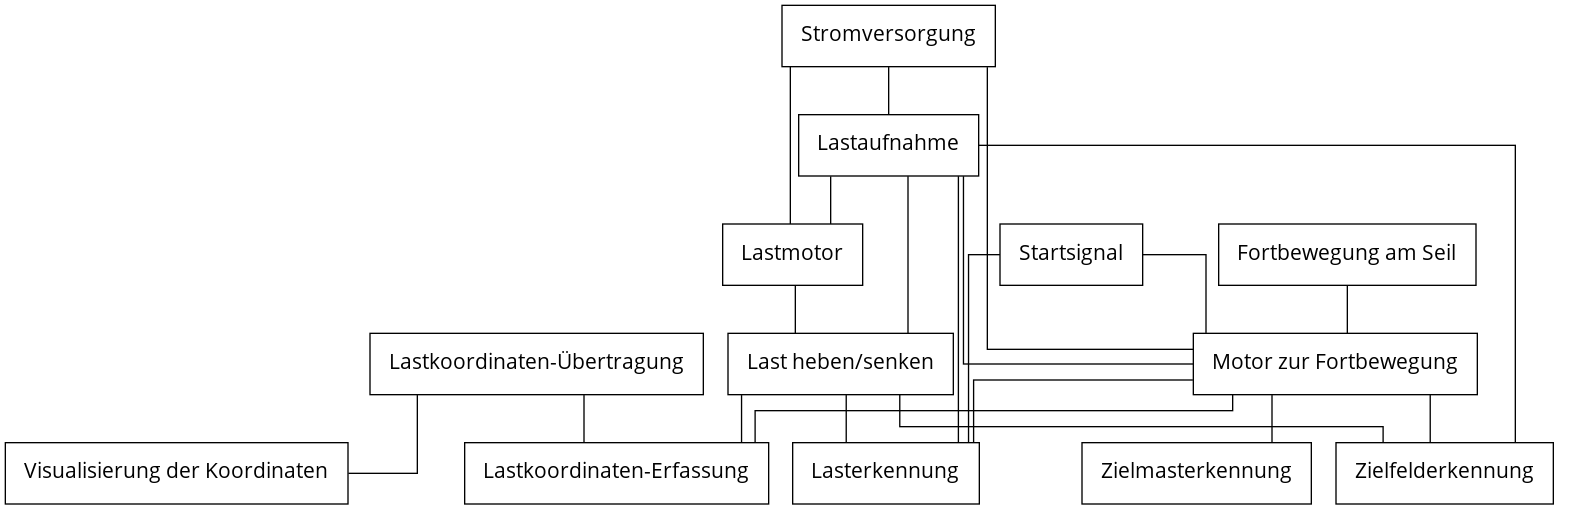
\includegraphics[width=\linewidth]{blockschaltbild.png}
    \caption{Funktionales Blockschaltbild}
    \label{fig:blockschaltbild}
\end{figure}

\subsection{Erläuterungen}

Die Stromversorgung speist den Lastmotor, die Lastaufnahme und den Motor zur Fortbewegung mit der benötigten Spannung.  Über ein Startsignal wird der Motor zur Fortbewegung gestartet. Damit beginnt die Fortbewegung am Seil, solange bis die Lasterkennung die Last erkennt und damit den Motor zur Fortbewegung vorübergehend stoppt.  Die Lastaufnahme greift die erkannte Last. Der Lastmotor wird benötigt um die erkannte Last zu heben.  Von nun an werden die Koordinaten der Last erfasst, zum Anwender übertragen und dort visualisiert. Somit weiss der Benutzer immer die genauen Koordinaten der Last.  Wenn die Last genug hoch gehoben wurde um keine Hindernisse mehr zu berühren wird der Motor zur Fortbewegung wieder gestartet.  Dieser Motor läuft solange bis die Zielfelderkennung das Zielfeld erkannt hat.  Nun stoppt der Antriebsmotor und der Lastmotor senkt die Last auf das Zielfeld wo die Lastaufnahme die Last loslässt und somit auf dem Zielfeld platziert. Sobald die Last abgeladen ist, startet der Motor zur Fortbewegung wieder bis die Zielmasterkennung durchgibt, dass der Zielmast erreicht wurde.

\newpage

\pagestyle{empty}

\begin{landscape}
\section{Anhang B: Morphologischer Kasten}
\label{lbl:MorphologischerKasten}

\newcommand{\rc}{\textcolor{red}{\large{\checkmark}}}
\newcommand{\gc}{\textcolor{green}{\large{\checkmark}}}

\def\arraystretch{1.5}
\begin{tabularx}{\hsize}{|X|p{15cm}|}
\hline
\large{\textsc{Komponente}} & \large{\textsc{Lösungsvarianten}} \\
\hline
Startsignal & Starttaste \hfill \gc Smartphone-App \hfill \rc Sprachsignal \hfill SSH-Befehl \hfill Webseite \\
Fortbewegung am Seil & \gc Reifen \hfill Raupe \hfill \rc Affenantrieb \hfill Luftdruck \hfill Propellerantrieb \\
Motor zur Fortbewegung & \rc \gc Schrittmotor \hfill Brushless-Motor \hfill Brushed-Motor \hfill Servomotor \\
Lasterkennung & \rc \gc Bilderkennung \hfill Drucktaster \hfill Ultraschallsensor \hfill Infrarotsensor \\
Lastaufnahme & Magnet \hfill mech. Greifer \hfill Vakuumglocke \hfill \rc \gc Softrobotics-Greifarm \hfill Lasso \\
Lastmotor & \rc \gc Schrittmotor \hfill Brushless-Motor \hfill Brushed-Motor \hfill Servomotor \\
Last heben/senken & \gc Seilzug \hfill Zahnstange \hfill Gewindestange \hfill \rc Telekopmast \hfill Nürnberger Schere \\
Zielfelderkennung & \gc Bilderkennung \hfill \rc Wärmebildkamera \hfill Infrarotsensor \hfill Reflektion messen \\
Stromversorgung & 9V-Batterie \hfill \gc Lithium-Polymer-Akku \hfill Bleiakku \hfill \rc Lithium-Ionen-Akku \\
Zielmasterkennung & \rc Bilderkennung \hfill \gc Drucktaster \hfill Ultraschallsensor \hfill Infrarotsensor \\
Lastkoordinaten-Erfassung & Infrarotsensor \hfill \gc Ultraschallsensor \hfill Schrittmotor \hfill \rc Bilderkennung \\
Lastkoordinaten-Übertragung & Bluetooth \hfill \gc WiFi \hfill Infrarot \hfill \rc Akustisch \\
Visualisierung der Koordinaten & Display auf Gerät \hfill \gc Smartphone-App \hfill \rc Desktop-Anwendung \hfill Webseite \\
\hline
\end{tabularx}
\rc Variante «High Tech» \hfill \gc Variante «optimiert»

\end{landscape}

\pagestyle{plain}

\newpage

\listoffigures

\end{document}
